
\documentclass[letterpaper, 10pt]{article}
\topmargin-2.0cm

\usepackage{fancyhdr}
\usepackage{hyperref}
\usepackage{lastpage}
\usepackage[dvips]{color}
\usepackage{graphicx}

% Color Information from -
% http://www-h.eng.cam.ac.uk/help/tpl/textprocessing/latex_advanced/node13.html

\advance\oddsidemargin-1in
\advance\evensidemargin-1.5cm
\textheight9.2in
\textwidth6.75in
\newcommand\bb[1]{\mbox{\em #1}}
\def\baselinestretch{1.05}

\newcommand{\hsp}{\hspace*{\parindent}}
\definecolor{gray}{rgb}{0.4,0.4,0.4}

\begin{document}
\thispagestyle{fancy}

% Leave Left and Right Header empty.
\lhead{}
\rhead{}

\renewcommand{\headrulewidth}{0pt} 
\renewcommand{\footrulewidth}{0pt} 

\fancyfoot[C]{\footnotesize
\textcolor{gray}{http://www.cs.columbia.edu/$\sim$jikk/application}} 

\pagestyle{fancy}
\lhead{\textcolor{gray}{\it Kangkook Jee}}
\rhead{\textcolor{gray}{\thepage /\pageref{LastPage}}}

% This kind of makes 10pt to 9 pt.
\begin{small}

%\vspace*{0.1cm}
\begin{center} {\LARGE \bf TEACHING STATEMENT}\\ \vspace*{0.1cm} {\normalsize
Kangkook Jee (jikk@cs.columbia.edu)} \end{center}
% Begin with my teaching philosophy.
University education should provide chances for student to cultivate their
potentials to succeed in their future careers as a competent computer science
professionals.  
%
As an CS educator, I focus on preparing students with principled understanding
about fundamental/theoretical CS topics along with known best practices both
from academia and industry for them to learn how to create reliable and
scalable products.

%I enjoy human interactions in the course of teaching.

\subsubsection*{In class teaching experiences}

During my PhD, I taught Comlumbia University's COMS3103-3: Programming Langauge
Python\footnote{\url{http://www.cs.columbia.edu/~jikk/teaching/3101-3/index.html}}.
%
% The course begin with 22 students and 14 students completed the course.  for
% failing to set appropriate level for assignment.
%
Although it was my first university level teaching experience, I enjoyed much
from the whole process of building a course from scratch, deliver prepared
materials, and making interactions with students.
% 
The course is largely composed of two distinct phases. The first one is about
language fundamentals while the second one focuses on specific topics/modules
relevant to student's interest. Establishing the latter was especially
challenging since the class comprised undergraduates, MS and PhD students from
diverse disciplines of CS, economics, philosophy, English literature and so on.
%
I began the semester surveying to know about students' expectation and the
background and I also attempted to maximize to face-to-face interaction with
each student throughout the semester.
% 
Students were to fulfill four homework assignments and a class project to
complete the course. 
%
Assignments were designed not only to assess student's comprehension about
course materials but also to introduce primitive CS concepts to non-major
students.
%
% basic data structures such as queue and stack as well as an algorithmic
% concept of TSP were used.
%
I also realized that it requires  substantial amount of time and effort to
write a new set of assignments each time given that students always can search
for solutions for recycled problems. 
%
Regarding a class project, students were to made teams of 3 $\sim$ 4 members to
conduct to a project relevant to their research interest.
%
It was an exciting experience to find out that many of project output were so
creative and reached out beyond my expectation.
%
% Some impressive example include search engine for Columbia university, NLP
% project that establishes character network extraction analyzing novel text
% done by English literature major.
%

Compensating for a challenging task of doing a class from the beginning to the
end, the course evaluation
result\footnote{\url{http://www.cs.columbia.edu/~jikk/teaching/3101-3/evaluation.html}}
performed by student were encouraging, especially for non-naive English speaker
as I am. In a nutshell, students rated 4.45/5 for overall quality of the course
and 4.64/5 for amount they learned from the class.

\subsubsection*{Designed courses} 

I have number of courses that I am outlining which I want to teach in near
future. First one is another language course about C++. Besides hugeness and
complications  It is holding a unique position in terms of efficiency
near-native performance and migration 

%Course that I'm capable of/interested in teaching.
As my major research interest lies in the area of system security utilizing 
techniques from number of core CS topics -- Programming language, Operating
system, and Security System architectures.

%\begin{figure}[tb]
%	\centering
%	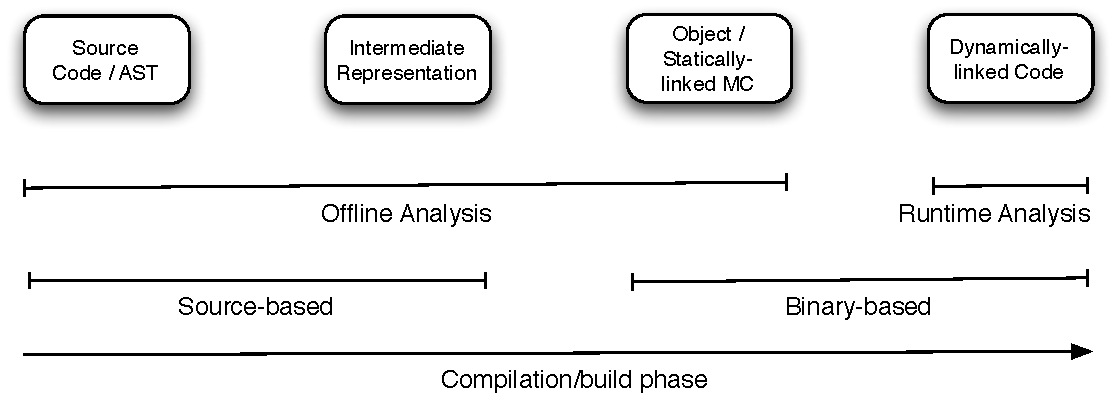
\includegraphics[width=0.5\linewidth]{figs/inst0.pdf}
%	\caption{Insturmentation}
%	\label{fig:decoupling}
%\end{figure}

I can teach wide ranges of CS core curriculum.
\begin{itemize}
\item Introduction to Computer Science
\item Programming language courses -- C, C++, Java, Python 
\item Senior level system courses -- desktop and mobile operating system,
  programming language.
\item Graduate level course: advanced compiler course -- instrumentation for
  software monitoring and protection.
\end{itemize}

Designing graduate level course 

\end{small}
\end{document}

